\section{Explain Your Code With Outputs}
\begin{figure}[h]
\centering
\footnotesize
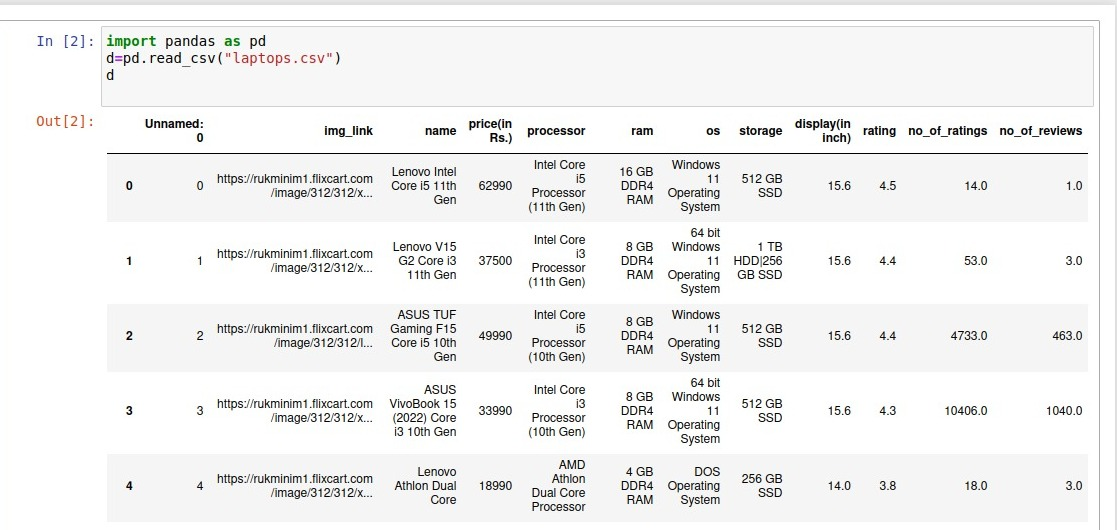
\includegraphics[width=7in]{20.jpeg}
\caption{csv file reading}
\label{fig:unevenlight}
\end{figure}

\vspace{4\baselineskip}
\begin{figure}[h]
\centering
\footnotesize
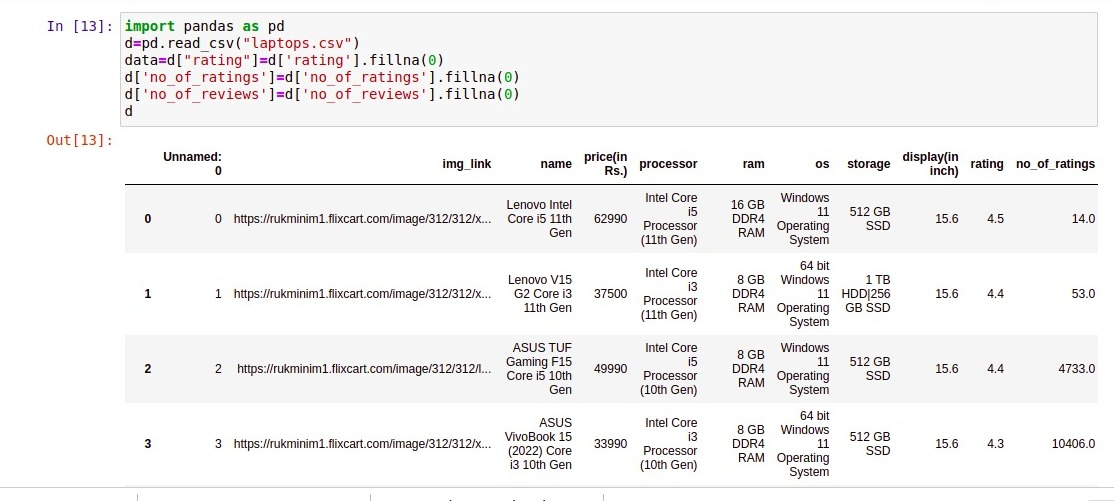
\includegraphics[width=6in]{21.jpeg}
\caption{filling the null values with 0}
\label{fig:unevenlight}
\end{figure}
\vspace{10\baselineskip}
\begin{figure}[h]
\centering
\footnotesize
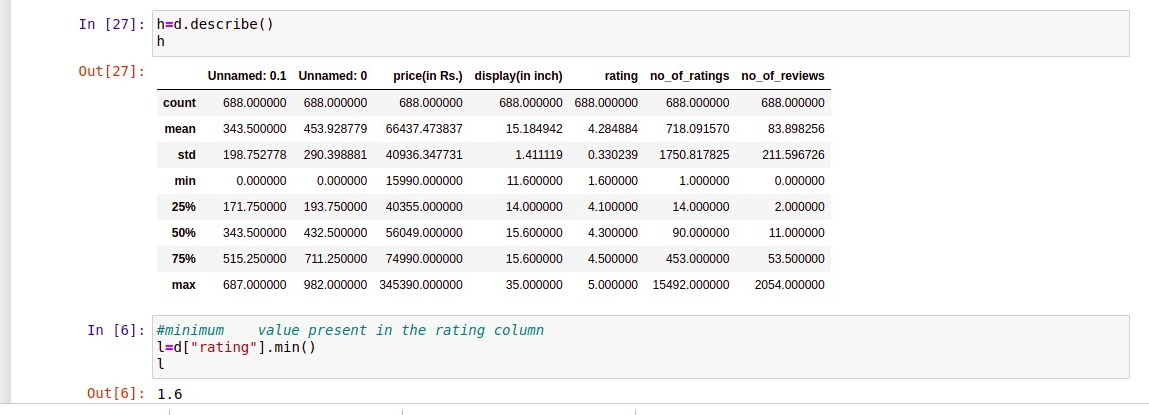
\includegraphics[width=9in]{22.jpeg}
\caption{stastical data}
\label{fig:unevenlight}
\end{figure}
\vspace{7\baselineskip}

\begin{figure}[h]
\centering
\footnotesize
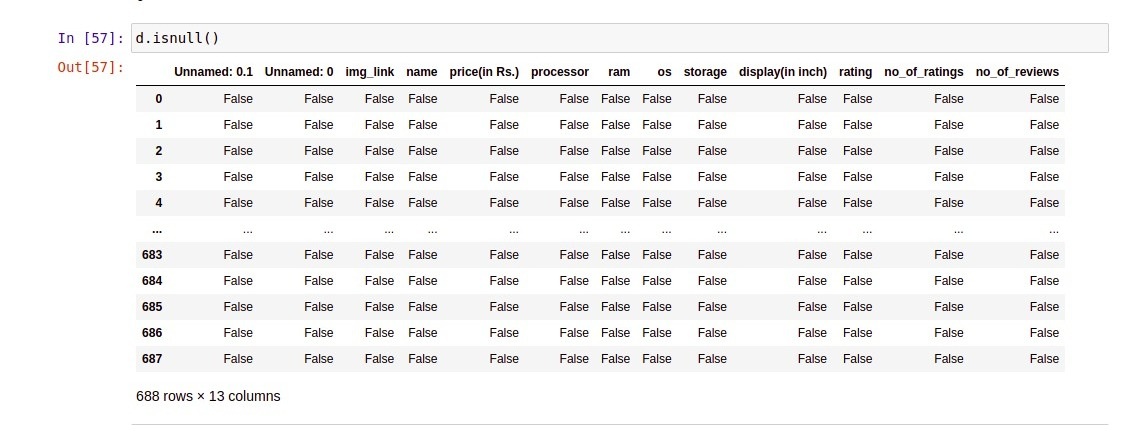
\includegraphics[width=7in]{23.jpeg}
\caption{finding Null values}
\label{fig:unevenlight}
\end{figure}
\vspace{7\baselineskip}

\begin{figure}[h]
\centering
\footnotesize
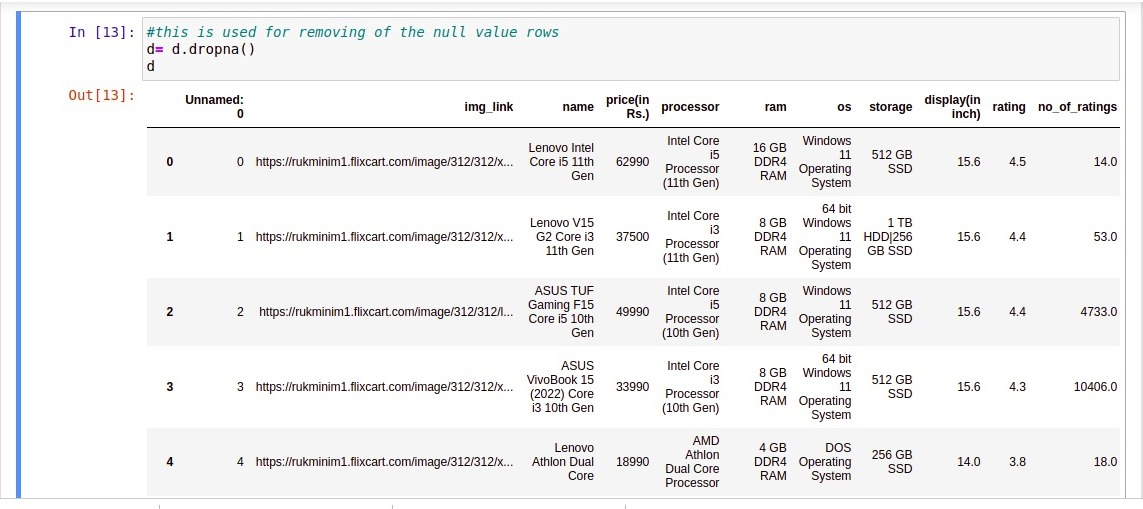
\includegraphics[width=7in]{28.jpeg}
\caption{Removing the null values containg rows}
\label{fig:unevenlight}
\end{figure}
\vspace{9\baselineskip}



\begin{figure}[h]
\centering
\footnotesize
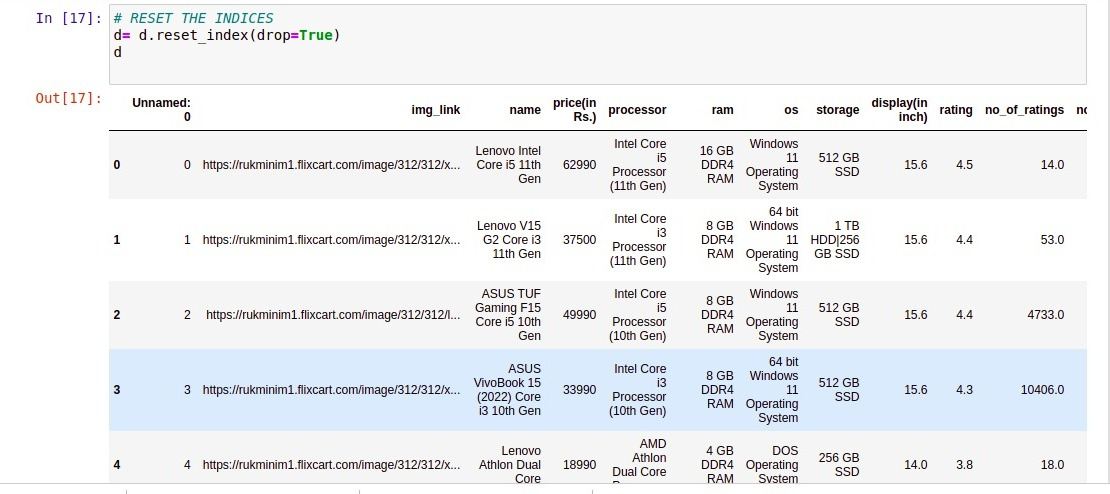
\includegraphics[width=7in]{29.jpeg}
\caption{Reset the indices}
\label{fig:unevenlight}
\end{figure}
\vspace{5\baselineskip}
\begin{figure}[h]
\centering
\footnotesize
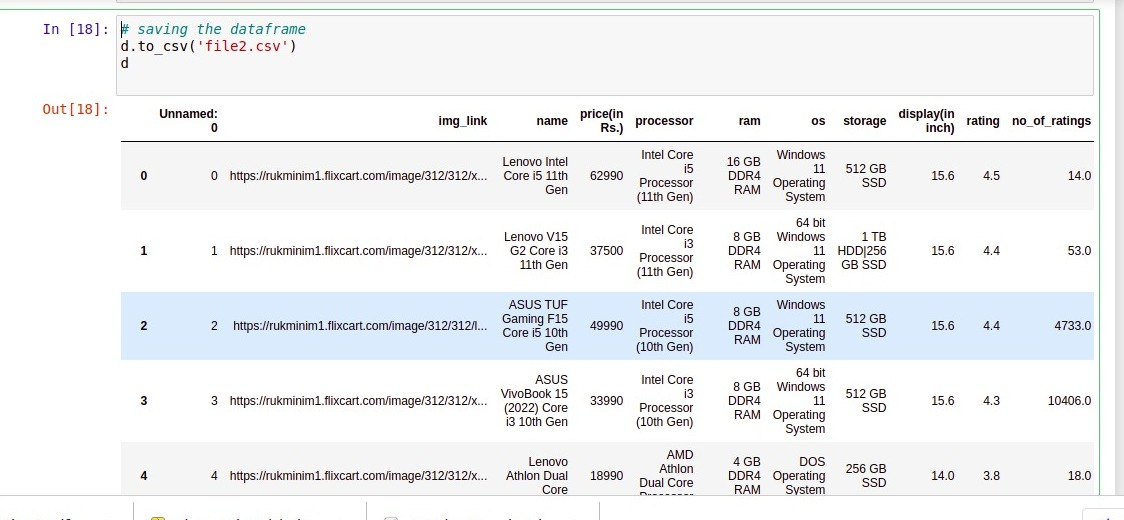
\includegraphics[width=6in]{30.jpeg}
\caption{After data processing saving dataframe into csv file }
\label{fig:unevenlight}
\end{figure}
\vspace{7\baselineskip}

\begin{figure}[h]
\centering
\footnotesize
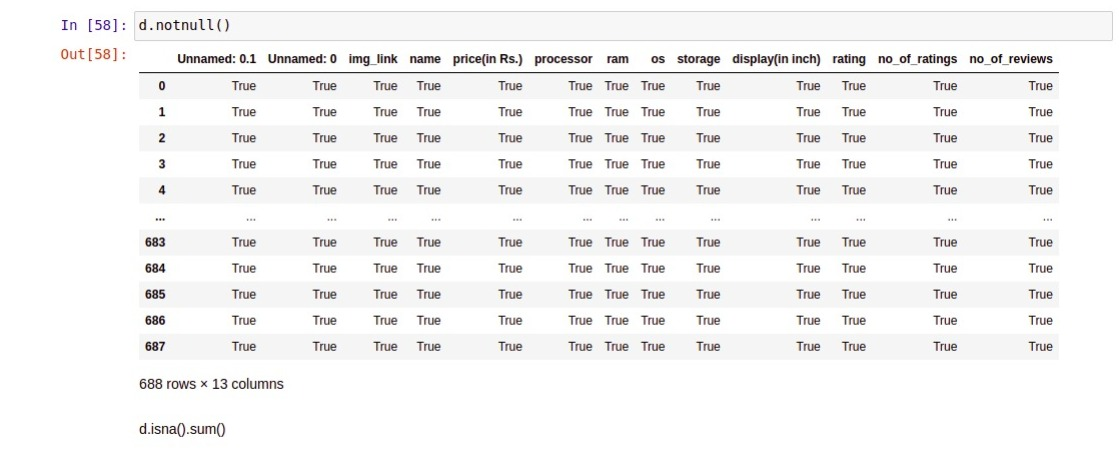
\includegraphics[width=7in]{24.jpeg}
\caption{checking the null values}
\label{fig:unevenlight}
\end{figure}

\begin{lstlisting}[language=Python]
import pandas as pd
import numpy as np
k=pd.read_csv("file2.csv")
k=pd.DataFrame(k)
k.sort_values(['price(in Rs.)'], inplace=True)
categorical_features =k.columns[(k.dtypes == 'object') == True].to_list()
print(categorical_features)
for feature in categorical_features:
    uniq = k[feature].unique()
    new_feature = []
    for el in k[feature]:
        new_feature.append(len(uniq) - np.where(uniq==el)[0][0])
    k[feature] = new_feature   
k
from sklearn.model_selection import train_test_split
from sklearn.ensemble import RandomForestClassifier
from sklearn.metrics import accuracy_score
from sklearn import metrics
from sklearn.metrics import mean_absolute_error, mean_squared_error, r2_score
import  matplotlib.pyplot as plt
import seaborn as sb
x=k.drop(['price(in Rs.)'], axis=1)
y=k["price(in Rs.)"].values
x_train, x_test, y_train, y_test = train_test_split(x, y, test_size=0.3, random_state=42)
rf_classifier = RandomForestClassifier(n_estimators=100)
rf_classifier.fit(x_train, y_train)
y_pred = rf_classifier.predict(x_test)
# Calculate accuracy
accuracy = accuracy_score(y_test, y_pred)
print("accuracy: ",accuracy)
MAE = mean_absolute_error(y_test, y_pred)
MSE = mean_squared_error(y_test, y_pred)
R2 = r2_score(y_test, y_pred)
print("Mean Absolute Error:", MAE)
print("Mean Squared Error:", MSE)
print("R-squared:", R2)
output:
\end{lstlisting}
\begin{figure}[h]
\centering
\footnotesize
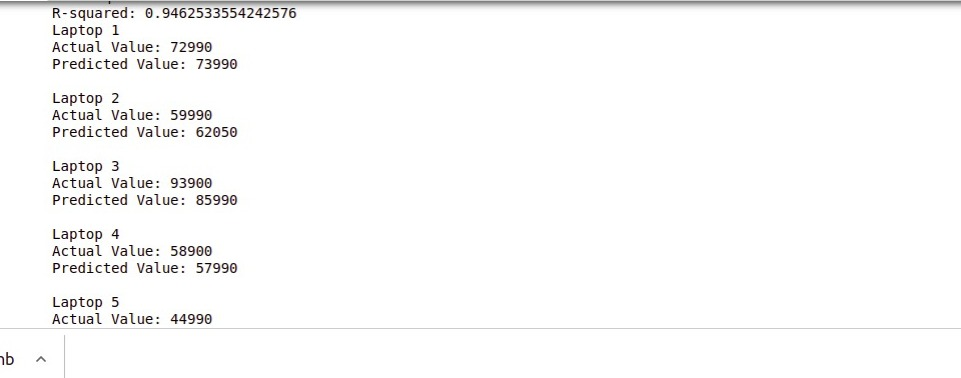
\includegraphics[width=6in]{56.jpeg}
\label{fig:unevenlight}
\end{figure}
\begin{lstlisting}[language=Python]
plt.scatter(y_test, y_pred)
plt.xlabel('Actual Values')
plt.ylabel('Predicted Values')
plt.title('Actual vs Predicted Values')
plt.show()
 \end{lstlisting} 
 output:    
\begin{figure}[h]
\centering
\footnotesize
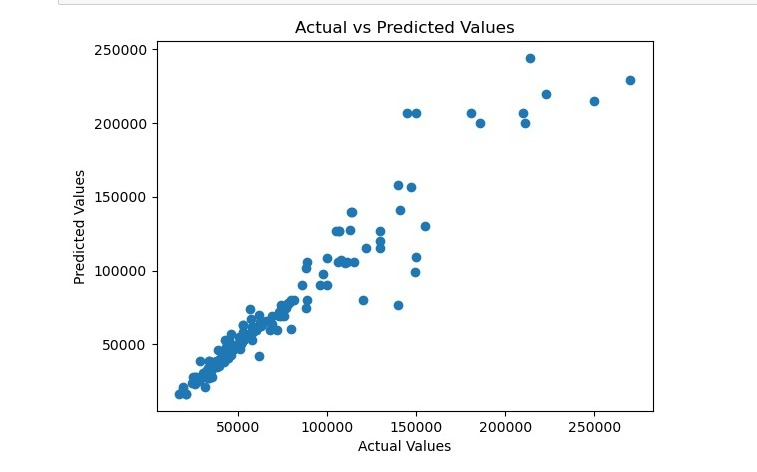
\includegraphics[width=5in]{35.jpeg}
\label{fig:unevenlight}
\end{figure}  

\begin{lstlisting}[language=Python]
\
plt.plot(range(len(y_test)), y_test, color='blue', label='Actual')
plt.plot(range(len(y_pred)), y_pred, color='red', label='Predicted')
plt.xlabel('Data Point Index')
plt.ylabel('Price')
plt.legend()
plt.show()
\end{lstlisting}
 \begin{figure}[h]
\centering
\footnotesize
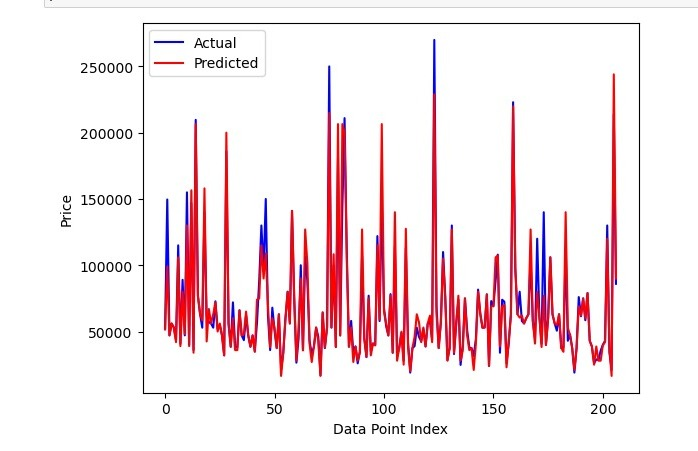
\includegraphics[width=3in]{31.png}
\caption{Actual vs Predicted values}
\label{fig:unevenlight}
\end{figure}
\vspace{2\baselineskip}
\begin{lstlisting}[language=Python]
plt.scatter(range(len(y_test)), y_test, color='blue', label='Actual')
plt.scatter(range(len(y_pred)), y_pred, color='red', label='Predicted')
plt.plot(range(len(y_pred)), y_pred, color='green', linewidth=2, label='Best Fit Line')
plt.xlabel('Data Point Index')
plt.ylabel('Price')
plt.legend()
plt.show()
\end{lstlisting}
output: 
\begin{figure}[h]
\centering
\footnotesize
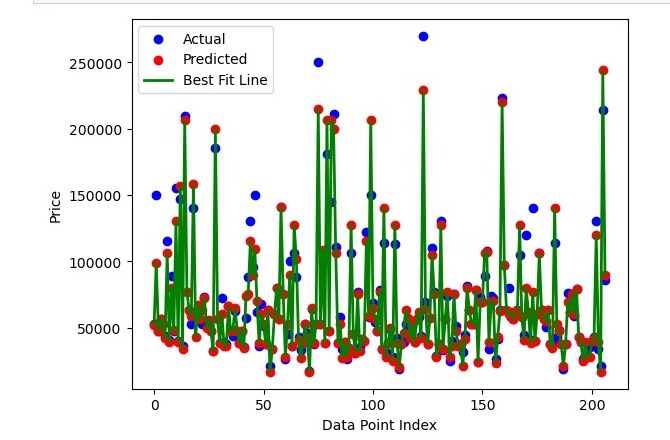
\includegraphics[width=6in]{33.jpeg}
\caption{Best Fit Line For Actual vs Predicted Values}
\label{fig:unevenlight}
\end{figure} 
 \begin{lstlisting}[language=Python]
plt.scatter(range(len(y_test)), y_test, color='blue', label='Actual')
plt.scatter(range(len(y_pred)), y_pred, color='red', label='Predicted')
plt.xlabel('Data Point Index')
plt.ylabel('Price')
plt.legend()
plt.show()
 \end{lstlisting} 
 output: 
 \begin{figure}[h]
\centering
\footnotesize
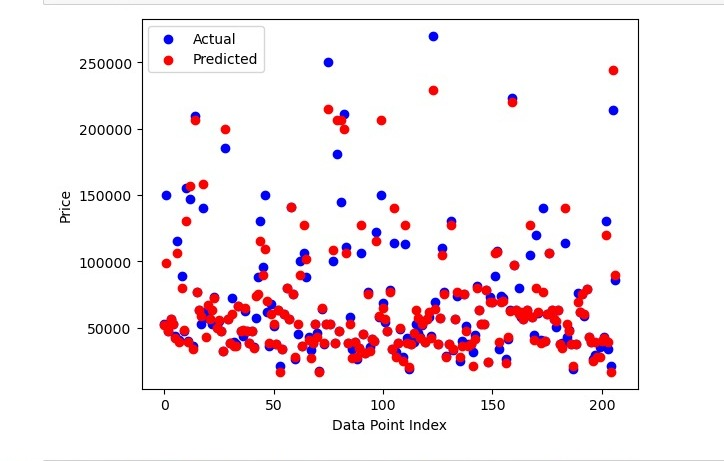
\includegraphics[width=4in]{34.jpeg}
\caption{scatter plot for  actual price vs predicted price }
\label{fig:unevenlight}
\end{figure}
\begin{lstlisting}[language=Python]
import pandas as pd
from sklearn.ensemble import RandomForestClassifier
k = pd.read_csv('file2.csv') 

categorical_features = k.columns[(k.dtypes == 'object') == True].to_list()
print(categorical_features)
for feature in categorical_features:
    uniq = k[feature].unique()

    new_feature = []
    for el in k[feature]:
        new_feature.append(len(uniq) - np.where(uniq == el)[0][0])

    k[feature] = new_feature

features = ['storage', 'ram', 'os'] 
target = 'name' 
X = k[features]
y = k[target]

rf_classifier = RandomForestClassifier(n_estimators=100)
rf_classifier.fit(X, y)

new_features = ["11", "15", "20"]
new_laptop = pd.DataFrame([new_features], columns=features)
prediction = rf_classifier.predict(new_laptop)
selected_laptop = k[k[target] == prediction[0]]

print("Selected Laptop:")
print(selected_laptop)
\end{lstlisting}
\begin{figure}[h]
\centering
\footnotesize
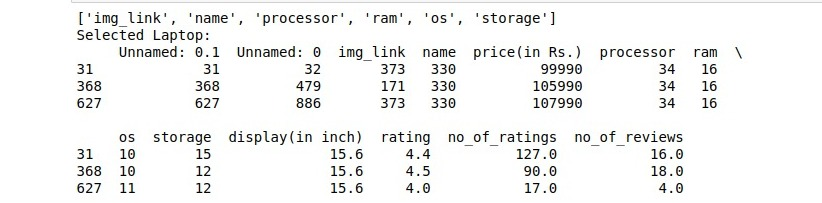
\includegraphics[width=5in]{54.jpeg}
\label{fig:unevenlight}
\end{figure}
\begin{lstlisting}[language=Python]
import pandas as pd
from sklearn.model_selection import train_test_split
from sklearn.ensemble import RandomForestRegressor
from sklearn.metrics import accuracy_score
from sklearn.metrics import mean_squared_error, r2_score
X=k.drop(['price(in Rs.)'], axis=1)
y=k["price(in Rs.)"].values
X_train, X_test, y_train, y_test = train_test_split(X, y, test_size=0.2, random_state=42)
rf = RandomForestRegressor()
rf.fit(X_train, y_train)
y_pred = rf.predict(X_test)
mse = mean_squared_error(y_test, y_pred)
r2 = r2_score(y_test, y_pred)
print('Mean Squared Error:', mse)
print('R-squared:', r2)
print("Actual values:")
print(y_test)
print("Predicted values:")
print(y_pred)
output:
R-squared value:0.9740704887906095
\end{lstlisting}





